\chapter{Program Verification}

\section{Test Runs}

\textbf{Five} or \textbf{six} different test runs are used to check new programs for accuracy and proper operation during execution.

During the execution of each of these six test runs, the control system detects fundamental programming errors, such as a cycle call with the spindle stopped or incorrect tangential points, etc.  
These errors are indicated on \textbf{line 3} of the screen by displaying the word \textbf{ERR} followed by an error code.

The meaning of the \textbf{error codes} is explained in an error list located inside the machine's control cabinet.

Detected programming errors \textbf{must} be eliminated immediately.

All six test runs can be performed in \textbf{SINGLE} and \textbf{AUTO} operation modes.

During the execution of these six tests, the following elements are activated:

\begin{itemize}
    \item Intervention keys affecting feed rate
    \item Intervention keys affecting the spindle
    \item Stop button for feed rate
    \item Stop button for feed rate of the leadscrew and main spindle
\end{itemize}

Test runs \textbf{1} and \textbf{2} are performed with axis movement (\textbf{MOTION}).

For these two test runs, the program is executed at a high feed rate, which is stored in the machine constants memory and can be modified using the intervention keys affecting the feed rate.

Axis movements can be stopped at any time by pressing the stop button for feed rate or the stop button for feed rate of the leadscrew and main spindle.

Test run \textbf{4} is performed without axis movement (\textbf{NO MOTION}).

However, axis movements can still be monitored on the visualization screen.

The test run \textbf{1} is a verification cycle with the \textbf{execution of machine functions} (\textbf{IO}).

During the execution of these cycles, the correct execution of auxiliary functions \textbf{M} can be monitored.

A displayed instruction for a \textbf{tool change} must be executed by pressing the \textbf{TOOL UNCL.} key twice to continue the verification cycle.

\marginnoteicon{20.8cm}{tool_uncl.jpg}

Test runs \textbf{2} and \textbf{4} are cycles \textbf{without the execution of machine functions} (\textbf{NO IO}).

\newpage
\section{Executing a Program Verification Cycle (TESTRUN)}

\begin{itemize}
    \item Search for the main program \textbf{P} to be verified (see section 7.1.1).
\end{itemize}

\begin{itemize}
    \iconitem{Press the \textbf{SINGLE} or \textbf{AUTO} key.}{single.jpg,auto.jpg}
\end{itemize}

\vspace{.5cm}

\begin{itemize}
    \iconitem{Press the \textbf{MENU} key.}{menu.jpg}
\end{itemize}

\vspace{.5cm}

The menu for selecting verification cycles (\textbf{TESTRUN 1...4}) appears on the screen:

\begin{center}
    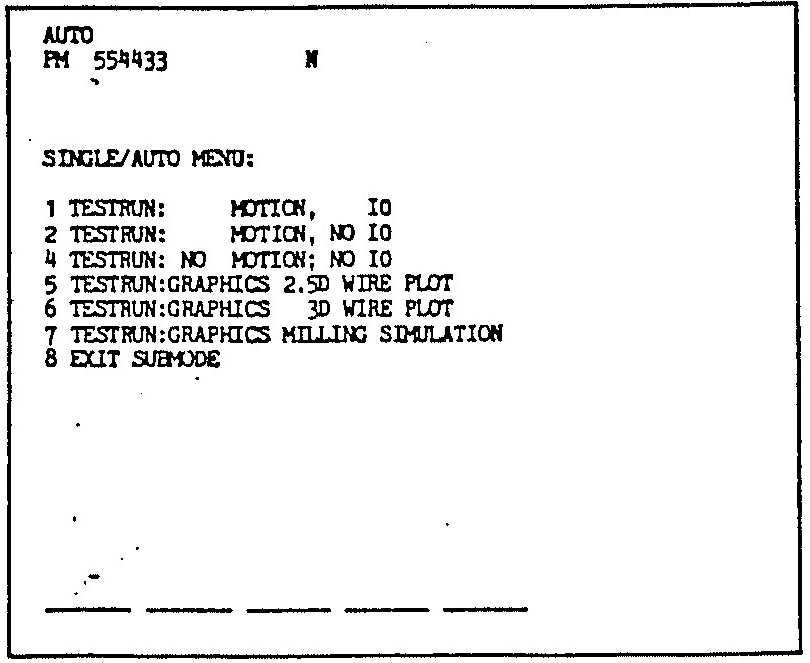
\includegraphics[width=0.7\textwidth]{testrun_menu.jpg}
\end{center}

\begin{itemize}
    \item Press the corresponding numeric key to select the desired verification cycle.
\end{itemize}

The first blocks of the program to be verified are displayed on the screen:

\begin{itemize}
    \item The indication \textbf{TESTRUN} followed by the selected verification cycle number is displayed on line 1 of the screen.
\end{itemize}

\begin{itemize}
    \iconitem{Press the \textbf{START} key to begin the verification cycle.}{start.jpg}
\end{itemize}
\vspace{.5cm}

Pressing the \textbf{START} key initializes the automatic verification cycle.

During the execution of the verification cycle in \textbf{SINGLE} mode, each block of the program to be verified is executed one by one. For this reason, the \textbf{START} key must be pressed again after each block.

\vspace{.5cm}
\textbf{Procedure to Follow in Case of a Programming Error Signal, see Sections 5.3 and 5.4}

After completing the verification cycle:

\begin{itemize}
    \iconitem{Press the \textbf{MANUAL} key.}{manual.jpg}
\end{itemize}
\vspace{.5cm}

\begin{itemize}
    \iconitem{Press the \textbf{AUTO} and \textbf{MENU} keys.}{auto.jpg,menu.jpg}
\end{itemize}
\vspace{.5cm}
\begin{itemize}
    \item Press the \textbf{8} key on the numeric keypad to cancel the test run.
\end{itemize}

The \textbf{TESTRUN} indication disappears from line 1 of the screen.

\newpage

\section{Program Control Cycle Interruption}

If a programming error is detected during the control cycle, the control cycle is interrupted, and an error signal is displayed.

To modify the erroneous program, it is necessary to interrupt the control cycle:

\begin{itemize}
    \iconitem{Press the \textbf{MANUAL} key.}{manual.jpg}
\end{itemize}
\vspace{.5cm}

\begin{itemize}
    \iconitem{Press the \textbf{CLEAR CONTR.} key.}{clear_contr.jpg}
\end{itemize}
\vspace{.5cm}

The detected error can then be eliminated by modifying the program.

\textbf{Modifying the program}, see section 6.2.

\begin{itemize}
    \iconitem{Clear the error signal by pressing the \textbf{CLEAR} key.}{clear.jpg}
\end{itemize}

\vspace{.5cm}

\section{Resuming the Program Control Cycle}

After modifying the program, the control cycle must be resumed:

\begin{itemize}
    \item Search for the information block \textbf{N} where the control cycle was interrupted (see section 7.1.2).
\end{itemize}

\begin{itemize}
    \iconitem{Press the \textbf{SINGLE} or \textbf{AUTO} key.}{single.jpg,auto.jpg}
\end{itemize}
\vspace{.5cm}

The indication \textbf{TESTRUN} followed by the selected control cycle number reappears on line 1 of the screen.

\begin{itemize}
    \iconitem{Press the \textbf{START} key.}{start.jpg}
\end{itemize}
\vspace{.5cm}

Continuation of the program control cycle.

\notes

If the program control cycle is not only abandoned (see section 5.3) but also canceled, it must be reselected (see section 5.2) before it can be resumed.

\newpage

\section{Test Runs Involving Graphical Representation}

Three test runs are available for representing a program graphically.

These are the following: graphical output for two and a half axes, graphical output for three axes, and a simulation graph that cannot be performed except with a color visualization screen.

To perform a graphical representation, certain conditions must be met in the first place.

First, it is necessary to enter all required data in the memory of the graphical parameters (see section 5.5.1).

If no entry has been made in block \textbf{NO} and in block \textbf{N2} of the graphical parameters, it is necessary to define within the program using function \textbf{G98 (=NO)} a visualization window and using function \textbf{G99 (N2)} a raw part.

For this purpose, it is necessary to switch to mode \textbf{PM} in block \textbf{N9} of the graphical parameters.

To enter the visualization window (G98) and the raw part (G99), specify the angle point \textbf{(XYZ)} located at the back left, viewed from the program origin point, along with the relative dimensions for the axes with \textbf{I, J, K}, viewed from the angle point.

\begin{center}
    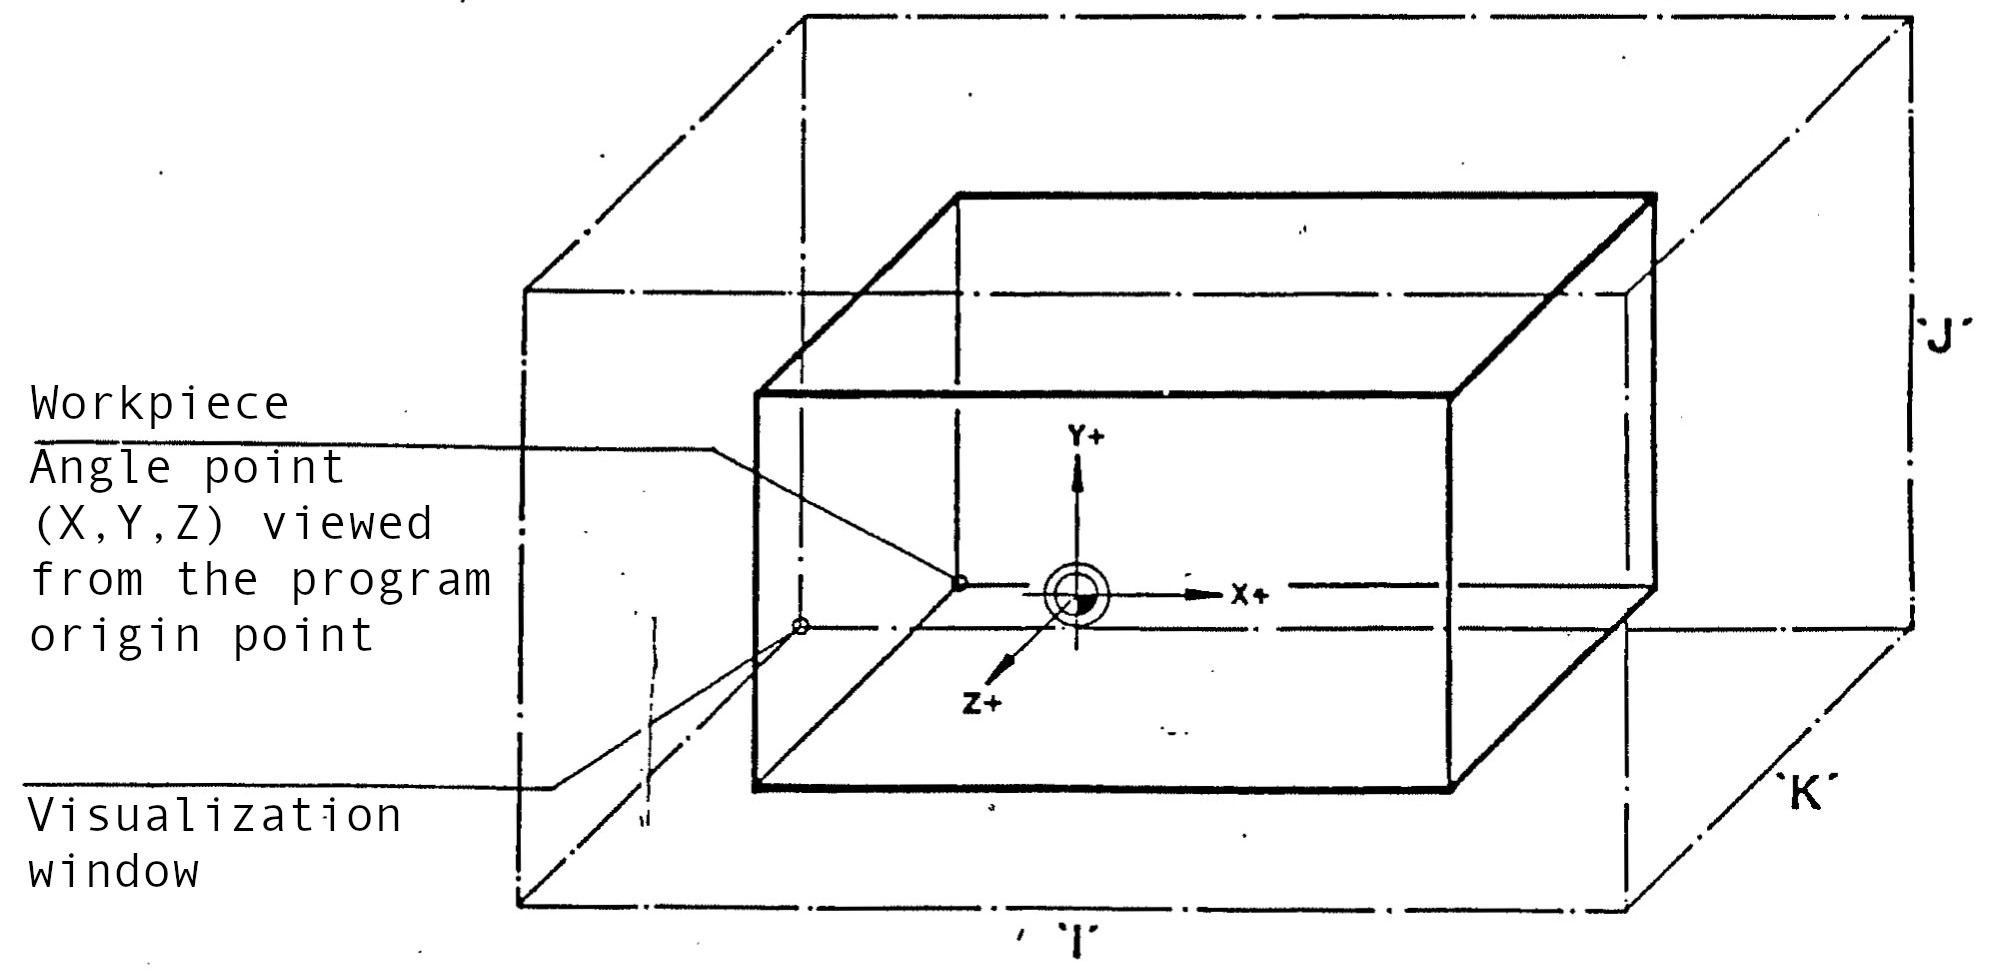
\includegraphics[width=0.8\textwidth]{graphical_dimensions.jpg}
\end{center}

\textbf{Indication of the window and raw part dimensions relative to the axes I, J, K, viewed from the angle point.}

\example{%
\begin{verbatim}
N1 G17 S1000 T1 M6
N2 G98 X-120 Y-120 Z-60 I240 J240 K60
N3 G98 X-100 Y-100 Z-50 I200 J200 K50
N4 G87 ...
\end{verbatim}
}

The program can contain up to \textbf{10 blocks} using function \textbf{G99} (asymmetric parts or clamping claws).  
To perform graphics output for three axes, it is necessary to enter two additional data values within the block using function \textbf{G98}.

\begin{itemize}
    \item \textbf{B..} = Rotation around the X-axis
    \item \textbf{B1..} = Rotation around the Y-axis
\end{itemize}

By using these two angle parameters, the workpiece can be visualized in any position in space.

\subsection{Graphic Parameters}

When selecting parameters (see section 5.5.2), their meaning is displayed each time in clear text  
(\textbf{DEFAULT = Power-on position}).

\underline{\textbf{N0}}

The visualization window can be entered using the reference graphic.

\procedure

\begin{itemize}
    \iconitem{Move the cursor to \textbf{NO}.}{up.jpg}
\end{itemize}

\vspace{.5cm}

\begin{itemize}
    \iconitem{Press the \textbf{F2} key (PICTURE).}{f2.jpg}
\end{itemize}

\vspace{.5cm}

The following image appears on the screen:

\begin{center}
    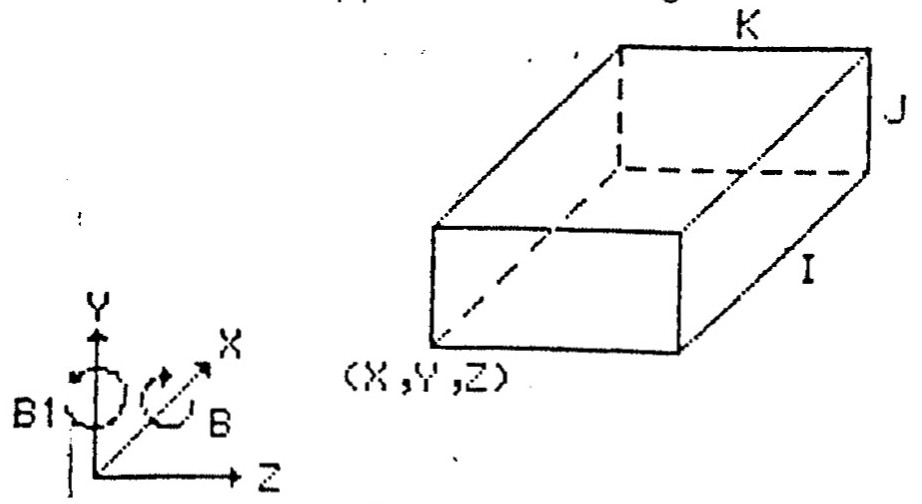
\includegraphics[width=0.6\textwidth]{graphic_window.jpg}
\end{center}

Return to the \textbf{GRAPHIC PARAMETER MENU} by pressing the \textbf{F4} function key (\textbf{PROGRAM}).

\notes

If no other value is introduced at this stage, a block with function \textbf{G98} must be programmed in the program after branching (\textbf{N9}) (see section 5.5).

\underline{\textbf{N1}}

By pressing the \textbf{F5 Cursor} function key (see section 5.5.3), the displayed image can be contracted or enlarged.  
The obtained dimensions are stored in the \textbf{WINDOW CURSOR}.

If the cursor is activated again, these values become the default for the visualization window.

\underline{\textbf{N2}}

The contour of the workpiece can be entered using reference graphics.

\newpage
\procedure

\begin{itemize}
    \iconitem{Move the cursor to \textbf{N2}.}{up.jpg,down.jpg}
\end{itemize}

\vspace{.5cm}

\begin{itemize}
    \iconitem{Press the \textbf{F2} key (PICTURE).}{f2.jpg}
\end{itemize}

\vspace{.5cm}

The following image appears on the screen:

\begin{center}
    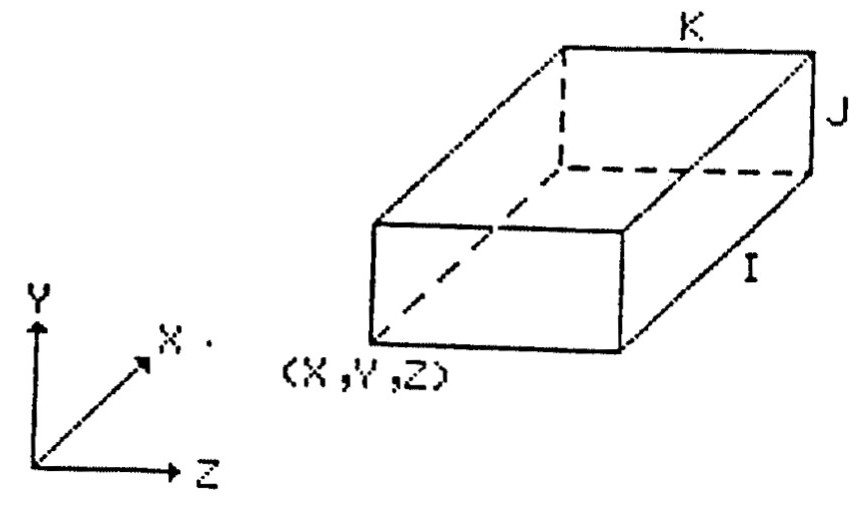
\includegraphics[width=0.6\textwidth]{graphic_outline.jpg}
\end{center}

\notes

If no other value is introduced at this stage, \textbf{at least one block} with function \textbf{G99} must be programmed in the program after branching (\textbf{N9}).

\underline{\textbf{N3}}

To graphically represent a specific \textbf{section} of the program, it is necessary to specify the \textbf{first and last block of this section} (similar to function \textbf{G14} for repetition).

\underline{\textbf{N4}}

Determination of the display of interruptions (e.g., program stop, tool change).

\textbf{Zero input:} Program stops are removed.

\underline{\textbf{N5}}

Timed stops.

\textbf{Zero input:} The timed stop is removed.

\underline{\textbf{N6}}

Final contour tracing.

\underline{\textbf{N7}}

Tracing of tool movements.

\underline{\textbf{N8}}

Projection method in case of representation of two and a half axes.  
European system or American system.

\underline{\textbf{N9}}

\textbf{Branching:}
\begin{tabbing}
    \hspace{1cm} \= NO/N2 is activated (GM) \\
    \> OR \\
    \> G98/G99 is activated (PM)
\end{tabbing}

\newpage
\subsection{Entering or Modifying Graphic Parameters}

\procedure

\begin{itemize}
    \iconitem{Press the \textbf{MANUAL} key.}{manual.jpg}
\end{itemize}

\vspace{.5cm}

\begin{itemize}
    \iconitem{Press the \textbf{PROG. MEM.} key.}{prog_mem.jpg}
\end{itemize}

\vspace{.5cm}

\begin{itemize}
    \iconitem{Press the \textbf{MENU} key.}{menu.jpg}
\end{itemize}

\vspace{.5cm}

The \textbf{PARTPROGRAM MENU} appears on the screen.

\begin{itemize}
    \item Enter the number \textbf{6} on the numeric keypad to select \textbf{GRAPHIC PARAMETERS}.
\end{itemize}

The list of graphic parameters appears on the screen:

\begin{center}
    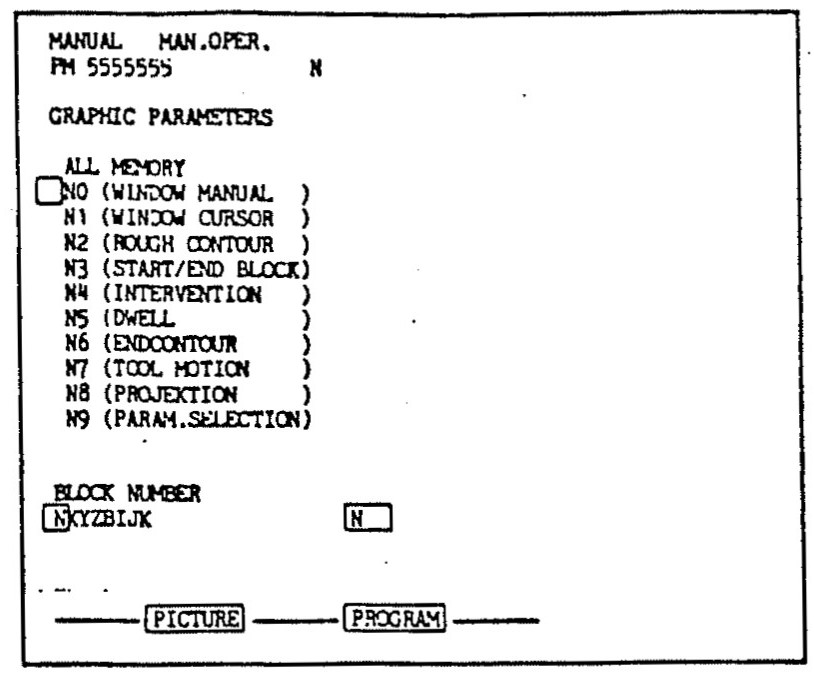
\includegraphics[width=0.7\textwidth]{graphic_parameters.jpg}
\end{center}

\begin{itemize}
    \iconitem{Select the block number of the parameter to be entered or modified by pressing the command keys \textbf{"up-down"}.}{up.jpg,down.jpg}
\end{itemize}

\vspace{.5cm}

\begin{itemize}
    \iconitem{Select the parameter to be entered by pressing the command keys \textbf{"left-right"}.}{left.jpg,right.jpg}
\end{itemize}

\vspace{.5cm}

\begin{itemize}
    \iconitem{Once the modification or entry is complete, press the \textbf{MANUAL} key.}{manual.jpg}
\end{itemize}

\newpage

\subsection{TESTRUN 5, Graphics for Two and a Half Axes, S. Plotter}

Selection of test runs, as described in section 5.2.

\begin{itemize}
    \item Enter the number \textbf{5} on the numeric keypad to select \textbf{graphics for two and a half axes, s. plotter}.
\end{itemize}

The \textbf{TESTRUN-5} indication then appears on \textbf{line 1} of the screen.

\begin{itemize}
    \iconitem{Press the \textbf{START} key.}{start.jpg}
\end{itemize}

\vspace{.5cm}

The current program is then displayed in \textbf{3 projection planes}.

\paragraph{Screen Display Process:}
\begin{enumerate}
    \item The coordinate system is drawn to scale.
    \item Views from the top, front, and side.
    \item Program execution:
    \begin{itemize}
        \item Rapid movement trajectories - \textbf{dashed lines}.
        \item Feed trajectories - \textbf{solid lines}.
    \end{itemize}
    \item The current coordinates (\textbf{X, Y, Z}) of the tool are displayed in the upper right corner of the screen.
\end{enumerate}

\subparagraph{Zooming In or Out on a Detail}

A specific detail can be selected using the \textbf{F5 (CURSOR)} function key.

\procedure

\begin{itemize}
    \iconitem{Press the \textbf{F5} function key (CURSOR).}{f5.jpg}
\end{itemize}

\vspace{.5cm}

A visualization window appears for each projection plane.

The following display appears on \textbf{line 24} of the screen:

\begin{center}
    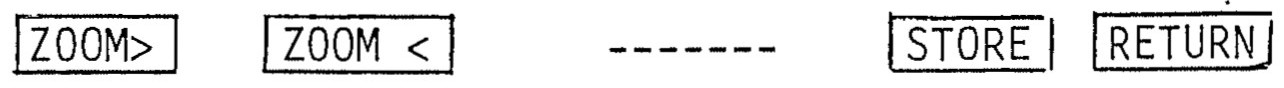
\includegraphics[width=0.8\textwidth]{zoom_store_return.jpg}
\end{center}

By pressing either function key \textbf{F1} (ZOOM >) or \textbf{F2} (ZOOM <), the visualization window can be enlarged or contracted.

By pressing the manual movement keys for the axes \textbf{-X, +X, -Y, +Y, -Z, +Z}, the visualization window can be shifted in the three indicated axes.

After setting the position and dimensions of the new window:

\begin{itemize}
    \iconitem{Press the \textbf{F2} function key (STORE).}{f2.jpg}
\end{itemize}

\vspace{.5cm}

The selected section is stored and can be checked under \textbf{N1} in the memory of the graphic parameters.

\begin{itemize}
    \iconitem{Press the \textbf{START} key.}{start.jpg}
\end{itemize}

\vspace{.5cm}

The reduced or enlarged section is now traced.

\notes

If another modification of the represented detail is necessary, the procedure must be repeated after a test run or after pressing the \textbf{STOP} key.

\paragraph{Reticle}

Any dimension of the graphic can be selected.  
Accuracy is determined based on the magnification level of the displayed image.

\procedure

At the end of the test run:

\begin{itemize}
    \iconitem{Press the \textbf{F4} function key (+).}{f4.jpg}
\end{itemize}

\vspace{.5cm}

A reticle appears on the screen for each projection plane.

To determine the dimensions, the reticle can be moved using the \textbf{MANUAL} keys:  
\textbf{+X, -X, +Y, -Y, +Z, -Z}.

The current coordinates of the reticle are displayed in the \textbf{upper right} part of the screen.

Pressing the \textbf{F5} (RETURN) key restores the previous operating state.

By pressing the \textbf{F2} (PRINT) key, the displayed image can be printed on a curve plotter.

\paragraph{To end the test run:}

\begin{itemize}
    \iconitem{Press the \textbf{MANUAL} key.}{manual.jpg}
\end{itemize}

\vspace{.5cm}

Enter the digit \textbf{8} via \textbf{AUTO}, \textbf{MENU} to cancel the test run.

\subsection{TESTRUN 6, Graphic Representation for Three Axes, s.plotter}

Selection of test runs, as described in section 5.2.

\begin{itemize}
    \iconitem{Press the \textbf{AUTO} key.}{auto.jpg}
\end{itemize}

\vspace{.5cm}

The \textbf{TESTRUN-6} indication appears on \textbf{line 1} of the screen.

\begin{itemize}
    \iconitem{Press the \textbf{START} key.}{start.jpg}
\end{itemize}

\vspace{.5cm}

\paragraph{On-screen execution:}

\begin{enumerate}
    \item The coordinate system \textbf{X, Y, Z} is plotted with the programmed rotation.
    \item The workpiece contour is displayed in perspective.
    \item The program runs as described for the \textbf{graphic representation for two and a half axes, s.plotter}.
    \item The current tool coordinates \textbf{X, Y, Z} are displayed on the \textbf{right side} of the screen.
\end{enumerate}

By pressing the \textbf{F2} (PRINT) key, the displayed image can be printed on a curve plotter.

\begin{itemize}
    \iconitem{Press the \textbf{MANUAL} key.}{manual.jpg}
\end{itemize}

\vspace{.5cm}

Enter the digit \textbf{8} via \textbf{AUTO}, \textbf{MENU} to cancel the test run.

\newpage

\subsection{TESTRUN 7, Simulation Graphics}

Selection of test runs, as described in section 5.2.

\begin{itemize}
    \iconitem{Press the \textbf{AUTO} key.}{auto.jpg}
\end{itemize}

\vspace{.5cm}

The \textbf{TESTRUN-7} indication is displayed on \textbf{line 1} of the screen.

\begin{itemize}
    \iconitem{Press the \textbf{START} key.}{start.jpg}
\end{itemize}

\vspace{.5cm}

The execution on the screen is identical to the one described in section \textbf{5.5.3}.

The use of functions \textbf{CURSOR}, \textbf{ZOOM >}, \textbf{ZOOM <}, \textbf{+}, and \textbf{RETURN} is identical to that of the graphical representation for two and a half axes, \textbf{s.plotter}.

\notes

In \textbf{simulation graphics} mode, it is possible to enable and disable the visualization of \textbf{collision states} and the \textbf{tool} by pressing the function keys \textbf{F4 (COLL-ON/OFF)} and \textbf{F5 (TOOL-ON/OFF)}.

The \textbf{cutting depths} are represented in different colors.